\documentclass[12pt, oneside]{article}
\usepackage{a4wide}
\usepackage{oldgerm}
\usepackage{amsmath}
\usepackage{amssymb}
\usepackage{amstext}
\usepackage{bm}
\usepackage{graphicx} 
\usepackage{tikz}
\usepackage{pgfplots}
\usepackage{booktabs}
\usepackage[super]{nth}
\setlength{\textheight}{8.875in} \setlength{\textwidth}{6.875in}
\setlength{\columnsep}{0.3125in} \setlength{\topmargin}{0in}
\setlength{\headheight}{0in} \setlength{\headsep}{0in}
\setlength{\parindent}{1pc} \setlength{\oddsidemargin}{-.304in}
\setlength{\evensidemargin}{-.304in}

\newcommand{\argmin}{\operatornamewithlimits{argmin}}
\allowdisplaybreaks

\graphicspath{ {./images/} }

\begin{document}
\setlength{\textheight}{8.5in}
\centering {\bf MTL 390 (Statistical Methods) }\\


\centering{\bf Minor Examination Assignment 1 Report}



\vskip 0.5cm

\noindent Name: Arpit Saxena ~  ~~~~~ ~~~~ ~~~~~~~~~~~~~~~~ Entry Number: 2018MT10742 ~~~~~~~~~~~~~



\vskip 0.5cm



\begin{enumerate}

\item	{
    Descriptive Statistics

    Consider data taken from a bivariate distribution which is listed in the following table:

    \begin{center}
      \begin{tabular}{cc}
      \toprule
        \(x_1\) &   \(x_2\) \\
      \midrule
      4.597941 & -0.082831 \\
      3.199353 &  1.097550 \\
      1.680648 &  0.410578 \\
      -1.885425 &  0.513452 \\
      -0.207406 & -1.094364 \\
      3.604727 & -0.528722 \\
      2.043016 &  0.232730 \\
      4.392772 & -0.806960 \\
      0.923505 & -3.016915 \\
      1.334248 &  0.789666 \\
      4.421921 & -0.763320 \\
      2.965662 &  1.642863 \\
      2.223469 & -2.652278 \\
      1.801136 &  1.881806 \\
      -2.200512 &  0.049598 \\
      \bottomrule
      \end{tabular}
    \end{center}

    Find the biased and unbiased sample covariance matrices for the given data. Using that,
    or otherwise, find the kurtosis and excess kurtosis of the given sample. Do the same
    thing treating each variable as an individual sample from a distribution.

    \textbf{Answer}

    Let \(\bm{x_1},\ldots,\bm{x_n}\) be \(n\) samples from the data, then the biased sample
    covariance matrix is given by:
    \begin{align*}
      S_1 &= \frac{1}{n} \sum_{i=1}^{n} \left[(\bm{x_i} - \bm{\overline{x}})(\bm{x_i} - \bm{\overline{x}})^T\right] \\
      \intertext{Now, substituting values from the given data and calculating, we get}
      S_1 &= \begin{bmatrix}
        4.174 & -0.018 \\
        -0.018 & 1.803
      \end{bmatrix} \\
      \intertext{Now, the unbiased matrix is given by}
      S_2 &= \frac{n}{n - 1} S_1 \\
        &= \frac{15}{14} S_1 \\
        &= \begin{bmatrix}
          4.472 & -0.019 \\
          -0.019 & 1.932
        \end{bmatrix}
    \end{align*}

    The sample kurtosis is then given by:
    \begin{align*}
      \text{Kurtosis} &= \frac{1}{n} \sum_{i=1}^{n} \left[(\bm{x_i} - \bm{\overline{x}})^T S_1^{-1} (\bm{x_i} - \bm{\overline{x}})\right]^2 \tag*{(From \cite{kurtpaper})} \\
      \intertext{We first calculate the sample mean from the data as:}
      \bm{\overline{x}} &= (1.926, -0.155)^T \\
      \intertext{Then, we calculate the kurtosis using the given formula and get}
      \text{Kurtosis} &= 5.93
    \end{align*}

    For a multivariate normal distribution distribution of \(p\) variables, the expected
    kurtosis is (from \cite{kurtpaper}) \(p(p + 2)\). Thus, the expected kurtosis for
    bivariate normal distribution is \(2 * 4 = 8\). Therefore, excess kurtosis equals 
    \(5.93 - 8 = -2.07\) and our given sample is mesokurtic.

    Treating the columns individually, we get

    \begin{center}
      \begin{tabular}{ccc}
        \toprule
        {} & Kurtosis & Excess Kurtosis \\
        \midrule
        \(x_1\) & 2.865 & -0.135 \\
        \(x_2\) & 3.302 & 0.302\\
        \bottomrule
      \end{tabular}
    \end{center}
}


\item	{
  Descriptive Statistics

  Given data is from world bank and contains values for the indicator ``Population ages 0-14
  (\% of population)" for some 15 randomly selected countries and for 3 years, namely: 2005,
  2010 and 2015. Visualize this data and draw observations.

  \begin{center}
    \begin{tabular}{lrrr}
      \toprule
      {} &       2005 &       2010 &       2015 \\
      Country Code &            &            &            \\
      \midrule
      KOR          &  18.827339 &  16.101602 &  13.781719 \\
      MEX          &  31.837208 &  29.507688 &  27.635969 \\
      BOL          &  36.326591 &  34.489515 &  32.404954 \\
      BDI          &  46.977947 &  45.140314 &  45.520683 \\
      VCT          &  28.554330 &  25.833449 &  23.719170 \\
      OSS          &  34.171454 &  31.320387 &  30.379485 \\
      SLB          &  41.314868 &  40.751637 &  40.430065 \\
      CUB          &  19.201050 &  17.741081 &  16.674866 \\
      HPC          &  45.152638 &  44.694382 &  43.648154 \\
      PNG          &  39.179415 &  38.302255 &  36.796778 \\
      VEN          &  31.689552 &  29.907486 &  28.380399 \\
      FJI          &  30.534296 &  29.000440 &  29.847679 \\
      NOR          &  19.612168 &  18.811563 &  17.962317 \\
      LTE          &  21.593859 &  19.838022 &  19.213434 \\
      SAU          &  33.873896 &  29.703454 &  25.822845 \\
      \bottomrule
      \end{tabular}
  \end{center}
  
  \textbf{Answer}

  The given data is basically showing changing of distributions over time. We can
  visualize one distribution by plotting a box plot and then we could plot multiple
  box plots over the years to see how this data varies.

  (The following plot was exported from python to tikz)

  \begin{center}
  % This file was created by tikzplotlib v0.9.8.
\begin{tikzpicture}

  \definecolor{color0}{rgb}{0.800490196078431,0.35343137254902,0.28578431372549}
  \definecolor{color1}{rgb}{0.271078431372549,0.524019607843137,0.674019607843137}
  \definecolor{color2}{rgb}{0.621078431372549,0.591666666666667,0.800490196078431}
  
  \begin{axis}[
  axis background/.style={fill=white!89.8039215686275!black},
  axis line style={white},
  tick align=outside,
  tick pos=left,
  x grid style={white},
  xlabel={Year},
  xmin=-0.5, xmax=2.5,
  xtick style={color=white!33.3333333333333!black},
  xtick={0,1,2},
  xticklabels={2005,2010,2015},
  y grid style={white},
  ylabel={Population ages 0-14 (\% of total population)},
  ymajorgrids,
  ymin=12.1219078577978, ymax=48.6377588573742,
  ytick style={color=white!33.3333333333333!black}
  ]
  \path [draw=white!28.2352941176471!black, fill=color0, semithick]
  (axis cs:-0.4,25.0740946066542)
  --(axis cs:0.4,25.0740946066542)
  --(axis cs:0.4,37.75300277905)
  --(axis cs:-0.4,37.75300277905)
  --(axis cs:-0.4,25.0740946066542)
  --cycle;
  \path [draw=white!28.2352941176471!black, fill=color1, semithick]
  (axis cs:0.6,22.8357353371206)
  --(axis cs:1.4,22.8357353371206)
  --(axis cs:1.4,36.3958849969844)
  --(axis cs:0.6,36.3958849969844)
  --(axis cs:0.6,22.8357353371206)
  --cycle;
  \path [draw=white!28.2352941176471!black, fill=color2, semithick]
  (axis cs:1.6,21.4663021291766)
  --(axis cs:2.4,21.4663021291766)
  --(axis cs:2.4,34.6008661709388)
  --(axis cs:1.6,34.6008661709388)
  --(axis cs:1.6,21.4663021291766)
  --cycle;
  \addplot [semithick, white!28.2352941176471!black]
  table {%
  0 25.0740946066542
  0 18.8273387734188
  };
  \addplot [semithick, white!28.2352941176471!black]
  table {%
  0 37.75300277905
  0 46.9779474483025
  };
  \addplot [semithick, white!28.2352941176471!black]
  table {%
  -0.2 18.8273387734188
  0.2 18.8273387734188
  };
  \addplot [semithick, white!28.2352941176471!black]
  table {%
  -0.2 46.9779474483025
  0.2 46.9779474483025
  };
  \addplot [semithick, white!28.2352941176471!black]
  table {%
  1 22.8357353371206
  1 16.101601763675
  };
  \addplot [semithick, white!28.2352941176471!black]
  table {%
  1 36.3958849969844
  1 45.140314182232
  };
  \addplot [semithick, white!28.2352941176471!black]
  table {%
  0.8 16.101601763675
  1.2 16.101601763675
  };
  \addplot [semithick, white!28.2352941176471!black]
  table {%
  0.8 45.140314182232
  1.2 45.140314182232
  };
  \addplot [semithick, white!28.2352941176471!black]
  table {%
  2 21.4663021291766
  2 13.7817192668695
  };
  \addplot [semithick, white!28.2352941176471!black]
  table {%
  2 34.6008661709388
  2 45.5206825176697
  };
  \addplot [semithick, white!28.2352941176471!black]
  table {%
  1.8 13.7817192668695
  2.2 13.7817192668695
  };
  \addplot [semithick, white!28.2352941176471!black]
  table {%
  1.8 45.5206825176697
  2.2 45.5206825176697
  };
  \addplot [semithick, white!28.2352941176471!black]
  table {%
  -0.4 31.8372080283644
  0.4 31.8372080283644
  };
  \addplot [semithick, white!28.2352941176471!black]
  table {%
  0.6 29.7034538021151
  1.4 29.7034538021151
  };
  \addplot [semithick, white!28.2352941176471!black]
  table {%
  1.6 28.3803986785511
  2.4 28.3803986785511
  };
  \end{axis}
  
  \end{tikzpicture}
\end{center}

  From the given box plots, we can observe that the mean percentage population aged
  0-14 has been creasing over the years. While the minimum value in this sample has
  been decreasing, the maximum value is roughly the same. Thus there is an increased
  variance in the value of this indicator. While there are some countries in which
  the percentage of children has come down (could indicate aging population) while
  in other countries of the world it has either increased or stayed the same.
  
}


\item	{
  Sampling Distributions

  At an organization, there are \(10\) systems and each one has a different processing
  power. Suppose there are \(10\) jobs whose loads (as defined by some metric) are
  randomly picked from the interval \((0, 100)\). One job is assigned to one system,
  and the assignment is done by arranging the systems and jobs in an increasing order
  (of processing power and load respectively) and assign each job to the system at 
  the same index in the other list.

  Find the probability distribution of the load at each system. Hence or otherwise, find
  the expected load of the job ending up on the third system (arranged in increasing order).

  \textbf{Answer}

  Let \(X_1, \ldots, X_{10}\) be samples from the distribution \(U(0, 1)\). Then
  \(100X_i \sim U(0, 100) \,\forall i = 1,\ldots,10 \) would represent the job loads.
  The ordering amongst \(X_i\)'s and \(100X_i\)'s is the same, so we work with \(X_i\)'s
  to make our life easier.

  Suppose \(X_i\)'s arranged in ascending order are \(X_{(1)}, X_{(2)}, \ldots, X_{(10)}\).

  Let \(k \in \{1, \ldots, 10\}\) and \(n = 10\). Also, let \(\epsilon > 0\) be small. Then:
  \begin{align*}
    P(X_{(k)} \in [x, x + \epsilon]) &= P(\text{one of \({X_1, \ldots, X_{10}}\) lies in \([x, x + \epsilon]\)} \\
                                     &  \text{~~~~~~~~~and exactly \(k-1\) are less than \(x\)}) \\
      \intertext{(Now using the fact that \(X_i\)'s are independent)}
      &= {n \choose 1} P(\text{one lies in \([x, x + \epsilon]\)}) P(\text{exactly \(k-1\) are less than \(x\)}) \\
      &= n \epsilon {{n - 1} \choose {k - 1}} P(X_1 \leq x)^{k-1} P(X_1 > x)^{n-k} \tag*{(Since pdf is \(f(x) = 1\))} \\
      &= n \epsilon \frac{(n - 1)!}{(k - 1)!\,(n-k)!} x^{k-1} (1-x)^{n-k} \\
    \implies f_{X_{(k)}}(x) &= \frac{ x^{k-1} (1-x)^{n-k}}{\frac{{(k - 1)!\,(n-k)!}}{n!}} \\
      &= \frac{x^{k-1} (1-x)^{n-k}}{\frac{\Gamma(k) \Gamma(n-k+1)}{\Gamma(n+1)}} \\
      &= \frac{x^{k-1} (1-x)^{n-k}}{B(k, n - k + 1)} \tag*{(where \(B\) is the Beta function)}
  \end{align*}

  We note that
  \[X \sim B(\alpha, \beta) \implies f_X(x) = \frac{x^{\alpha - 1}(1-x)^{\beta - 1}}{B(\alpha, \beta)}\]
  where \(B(\cdot, \cdot)\) is the Beta-distribution.

  Comparing the equations of Beta distribution's pdf and the pdf we obtained for \(X_{(k)}\), we
  conclude that \[X_{(k)} \sim B(k, n - k + 1) \,\forall k \in \{1, \ldots, 10\}\]

  Now, we find the expected value of \(X_{(3)}\) as:
  \begin{align*}
    E(X_{(k)}) &= \int_{0}^{1} x \times \frac{x^{k-1} (1-x)^{n-k}}{B(k, n - k + 1)} dx \\
    \implies E(X_{(3)}) &= \int_{0}^{1} x \times \frac{x^{2} (1-x)^{8}}{B(3, 8)} dx \tag*{(\(\because n = 10\))} \\
      &= \frac{1}{B(3, 8)} \int_{0}^{1} x^3 (1 - x)^8 dx \\
      &= \frac{1}{B(3, 8)} \int_{0}^{1} (1 - x)^3 x^8 dx \\
      &= \frac{1}{B(3, 8)} \int_{0}^{1} x^8 (1 - 3x + 3x^2 - x^3) dx \\
      &= \frac{\Gamma(11)}{\Gamma(3)\Gamma(8)} \int_{0}^{1} (x^8 - 3x^9 + 3x^{10} - x^{11}) dx \\
      &= \frac{10!}{2!\,7!} \left[\frac{1}{9} - \frac{3}{10} + \frac{3}{11} - \frac{1}{12}\right] \\
      &= 360 \left[ \frac{1}{36} - \frac{3}{110} \right] \\
      &= 0.182
  \end{align*}

  Therefore, the expected load of the job ending up at the \nth{3} system is \(100E(X_{(k)}) = 18.2\)
}



\item	{
  Sampling Distributions 

  Consider that any insurance claim can be modelled as coming from an exponential distribution.
  Two companies had 30 insurance claims over some period of time. Suppose that claims for the
  companies come from exponential distributions with means 10 and 12 (in lakhs) respectively.
  Then what is the probability that total insurance claims made to company 1 are greater than
  claims made to company 2? Solve this using two different approaches and compare answers.

  \textbf{Answer}

  Insurance claims to companies 1 and 2 are distributed as Exp\((\frac{1}{10})\) and 
  Exp\((\frac{1}{12})\) respectively.

  Then one approach could be that sum of all insurance claims would be distributed as
  Gamma(\(30, \frac{1}{10}\)) and Gamma(\(30, \frac{1}{12}\)) for company 1 and company 2
  respectively. Let \(X \sim \text{Gamma}(n, \lambda_1)\), \(Y \sim \text{Gamma}(n, \lambda_2)\)
  where \(n = 30, \lambda_1 = \frac{1}{10}, \lambda_2 = \frac{1}{12}\). Then,
  \begin{align*}
    P(X > Y) &= \int_{y=0}^{\infty} \int_{x=y}^{\infty} f_X(x) f_Y(y) \,dx \,dy \\
      &= \int_{0}^{\infty} f_Y(y) \int_{y}^{\infty} f_X(x) \,dx \,dy \\
      &= \int_{0}^\infty \frac{\lambda_2^n y^{n-1} e^{-\lambda_2 y}}{\Gamma(n)} \frac{\Gamma(n, \lambda_1 y)}{\Gamma(n)} dy \tag*{(where \(\Gamma(\cdot, \cdot)\) is the upper incomplete Gamma function)} \\
      &= \int_{0}^\infty \frac{\left(\frac{1}{12}\right)^{30} y^{29} e^{-\frac{y}{12}}}{29!} \frac{\Gamma(30, \frac{y}{10})}{29!} dy
  \end{align*}

  Now, solving using mathematical computational tools, we get
  \begin{equation}
    P(X > Y) = 0.2411 \label{eq:1}
  \end{equation}

  The other approach is that since the exponentially distributed random variables are
  iid and there are 30 of them, we can use CLT to approximate their sum. Claims for
  first company have mean \(10\) and variance \(10^2 = 100\), for the second company
  they have mean \(12\) and variance \(12^2 = 144\). Let \(\overline{X}, \overline{Y}\) be random variables
  denoting sample average claims made to companies 1 and 2 respectively.

  Then, by CLT we have:
  \begin{align*}
    \frac{\overline{X} - 10}{\frac{10}{\sqrt{30}}} &\sim \mathcal{N}(0, 1) \\
    \frac{\overline{Y} - 12}{\frac{12}{\sqrt{30}}} &\sim \mathcal{N}(0, 1) \\
  \end{align*}

  Let \(Z_1 = \frac{\overline{X} - 10}{\frac{10}{\sqrt{30}}}\) and \(Z_2 = \frac{\overline{Y} - 12}{\frac{12}{\sqrt{30}}}\).
  Then \(Z_1, Z_2\) are standard normal random variables and are also independent since
  they are made of samples which are independent. Now,
  \begin{align*}
    \overline{X} &> \overline{Y} \\
    \implies \frac{\overline{X} - 10}{\frac{10}{\sqrt{30}}} \frac{10}{\sqrt{30}} + 10 &> \frac{\overline{Y} - 12}{\frac{12}{\sqrt{30}}} \frac{12}{\sqrt{30}} + 12 \\
    \implies {\frac{10}{\sqrt{30}}} Z_1 + 10 &> \frac{12}{\sqrt{30}} Z_2 + 12 \\
    \implies \frac{10Z_1 - 12Z_2}{\sqrt{30}} &> 2 \\
    \implies Z_1 &> \frac{2\sqrt{30} + 12Z_2}{10}
  \end{align*}
  \begin{align*}
    \therefore P(\overline{X} > \overline{Y}) &= P\left(Z_1 > \frac{2\sqrt{30} + 12Z_2}{10}\right) \\
      &= \int_{z_2=-\infty}^{\infty} \int_{z_1 = \frac{2\sqrt{30} + 12z_2}{10}}^{\infty} f_{Z_2}(z_2) f_{Z_1}(z_1) dz_1 dz_2 \\
      &= \int_{-\infty}^{\infty} f_{Z_2}(z_2) \int_{z_1 = \frac{2\sqrt{30} + 12z_2}{10}}^{\infty}  f_{Z_1}(z_1) dz_1 dz_2 \\
      &= \int_{-\infty}^{\infty} f_{Z_2}(z_2) \left\{1 - \Phi\left(\frac{2\sqrt{30} + 12z_2}{10}\right)\right\} dz_2 \tag*{(where \(\Phi\) is the standard normal CDF)} \\
      &= \int_{-\infty}^{\infty} f_{Z_2}(z_2) \left\{\frac{1}{2} - \frac{1}{2}\text{erf}\left(\frac{2\sqrt{30} + 12z_2}{10\sqrt{2}}\right)\right\} dz_2
          \tag*{(Where erf is the Gauss error function)} \\
      &= \int_{-\infty}^{\infty} \frac{1}{\sqrt{2\pi}} e^{-\frac{z_2^2}{2}} \left\{\frac{1}{2} - \frac{1}{2}\text{erf}\left(\frac{2\sqrt{30} + 12z_2}{10\sqrt{2}}\right)\right\} dz_2
  \end{align*}

  The conversion from \(\Phi\) to erf helps us in using computational tools, which give the result as:
  \begin{equation}
    P(\overline{X} > \overline{Y}) = 0.2416 \label{eq:2}
  \end{equation}

  Now comparing (\ref{eq:1}) and (\ref{eq:2}), we observe the probabilities computes as 0.2411
  and 0.2416 and these probabilities are very close.
}


\item	{
  Point and Interval Estimations

  For a distribution with \(k\) unknown parameters, method of moments uses \(k\) moments
  to form a system of equations and solves it to find estimates for the parameters.
  This throws away information contained in higher order moments. To remedy that, the
  \textbf{Generalized Method of Moments (GMM)} takes \(q (> k)\) moments and minimizes
  the sum of squares of difference between sample moments and moments calculated from
  the distribution.

  Consider the following samples taken from a Poisson distribution with unknown \(\lambda\).
  Find an estimate for the parameter using both method of moments as well as generalized
  method of moments (with 3 moments)

  \begin{center}
  \begin{tabular}{cccc}
    \toprule
    30 & 21 & 24 & 18 \\
    28 & 25 & 24 & 25 \\
    26 & 19 & 19 & 21 \\
    22 & 34 & 22 & 15 \\
    22 & 25 & 16 & 22 \\
    \bottomrule
  \end{tabular}
  \end{center}

  \textbf{Answer}

  We first calculate expressions of three moments \(E[X], E[X^2] \text{ and } E[X^3]\) for
  \(X \sim P(\lambda)\).

  Using the MGF of the Poisson distribution, we find moments around 0:
  \begin{align*}
    M_X(t) &= exp(\lambda(e^t - 1)) \\
    \implies M_X'(t) &= \lambda e^t exp(\lambda e^t - \lambda) \\
    \implies M_X''(t) &= (\lambda e^t)^2 exp(\lambda e^t - \lambda) + \lambda e^t exp(\lambda e^t - \lambda) \\
    \implies M_X'''(t) &= (\lambda e^t)^3 exp(\lambda e^t - \lambda) + 2 (\lambda e^t)^2 exp(\lambda e^t - \lambda) \\
        &+ (\lambda e^t)^2 exp(\lambda e^t - \lambda) + \lambda e^t exp(\lambda e^t - \lambda) \\
        &= (\lambda e^t)^3 exp(\lambda e^t - \lambda) + 3 (\lambda e^t)^2 exp(\lambda e^t - \lambda) + \lambda e^t exp(\lambda e^t - \lambda) \\
  \end{align*}

  Using these, we calculate the moments as:
  \begin{align*}
    E[X] &= M_X'(0) = \lambda \\
    E[X^2] &= M_X''(0) = \lambda^2 + \lambda \\
    E[X^3] &= M_X'''(0) = \lambda^3 + 3\lambda^2 + \lambda
  \end{align*}

  Next we calculate the sample moments. Let the samples be written as \(x_1, ..., x_{20}\). Then:
  \begin{align*}
    m_1 &= \sum_{i=1}^{20} x_i  = 22.9\\
    m_2 &= \sum_{i=1}^{20} {x_i}^2 = 544.4 \\
    m_3 &= \sum_{i=1}^{20} {x_i}^3 = 13424.5 \\
  \end{align*}

  Using the method of moments, we get:
  \[\widehat{\lambda}_1 = m_1 = 22.9\]

  For the generalized method of moments, we note that we can take any weighting of the
  sample moments. In fact we can also take a positive definite matrix and define the
  cost function that way. Suppose we somehow decided to keep the weights for \(m_1, m_2, m_3\)
  to be \(100, 10, 1\) respectively. Then, we have the function:

  \begin{align*}
    Q(\lambda) &= 100(m_1 - E[X])^2 + 10(m_2 - E[X^2])^2 + 1(m_3 - E[X^3])^2 \\
               &= 100(22.9 - \lambda)^2 + 10(544.4 - \lambda^2 - \lambda)^2 + (13424.5 - \lambda^3 - 3\lambda^2 - \lambda)^2
  \end{align*}

  Then the estimator is given by:
  \[\widehat{\lambda}_2 = \argmin_\lambda{Q(\lambda)}\]

  We note that \(Q(\lambda)\) is a polynomial in lambda with degree 6, so it's not practical
  to calculate the minimum by hand. Using computer tools, we find:

  \[\widehat{\lambda}_2 = 22.79\]
}


\item	{
  Point and Interval Estimations

  Find an unbiased estimator for the parameter \(\lambda\) of an exponential 
  distribution Exp(\(\lambda\)) as a multiple of the sample mean. Given that the
  estimator found is the UMVUE, show that it does not achieve
  equality in the Cramer-Rao inequality, consequently showing that achieving the
  Cramer Rao Lower Bound is not a necessary condition for being UMVUE.

  Customers arrive at a checkout counter with an average time of 10 minutes as observed
  from 30 customers.
  What is the time in which their order should be processed so that 70\% of the customers
  don't find a line at the checkout counter.
  
  \textbf{Answer}

  Let \(X_1, \ldots, X_n \sim \text{Exp}(\lambda)\) be \(n\) samples from an exponential
  distribution with parameter \(\lambda\). Now, let

  \begin{align*}
    T(X) &= \frac{c}{\overline{X}} \\
         &= \frac{cn}{\sum_{i=1}^{n} X_i}
  \end{align*}

  Using the fact that sum of exponentially distributed variables follows the Gamma distribution,
  we define \(Z = \sum_{i = 1}^{n} X_i\) and note that \(Z \sim \text{Gamma}(n, \lambda)\).
  Then \(T(X) = \frac{cn}{Z}\)

  \begin{align*}
    E(T(X)) &= E\left(\frac{cn}{Z}\right) \\
            &= cn E\left(\frac{1}{Z}\right) \\
            &= cn \int_{0}^{\infty} \frac{1}{z} \frac{\lambda^n z^{n-1} e^{-\lambda z}}{\Gamma(n)} dz \tag*{(\(\because Z \sim Gamma(n, \lambda)\))} \\
            &= \frac{cn\lambda}{n-1} \underbrace{\int_{0}^{\infty} \frac{\lambda^{n-1} z^{n-2} e^{-\lambda z}}{\Gamma(n-1)} dz}_{ = 1} \tag*{(\(\because \Gamma(n) = (n-1) \Gamma(n-1)\))} \\
            &= \frac{cn\lambda}{n-1}
  \end{align*}

  To make this estimator unbiased, we have
  \begin{align*}
    E(T(X)) &= \lambda \\
    \implies \frac{cn\lambda}{n-1} &= \lambda \\
    \implies c &= \frac{n-1}{n} \\
    \therefore T(X) &= \frac{n - 1}{\sum_{i=1}^{n} X_i} \tag*{Since \(T(X) = \frac{cn}{\sum_{i=1}^{n} X_i}\)}
  \end{align*}

  Thus, we have found an unbiased estimator for T(X).

  Now, for Cramer-Rao inequality:

  \begin{align*}
    E\left(T(X)^2\right) &= E\left(\left(\frac{n-1}{\sum_{i=1}^{n} X_i}\right)^2\right) \\
      &= (n - 1)^2 E\left(\frac{1}{Z^2}\right) \\
      &= (n - 1)^2 \int_{0}^{\infty} \frac{1}{z^2} \frac{\lambda^n z^{n-1} e^{-\lambda z}}{\Gamma(n)} dz \tag*{(\(\because Z \sim \text{Gamma}(n, \lambda)\))} \\
      &= \frac{(n - 1)^2 \lambda^2}{(n - 1)(n - 2)}\underbrace{\int_{0}^{\infty}\frac{\lambda^{n-2} z^{n-3} e^{-\lambda z}}{\Gamma(n-2)} dz}_{=1} \tag*{(\(\because \Gamma(n) = (n-1) \Gamma(n-1)\))} \\
      &= \frac{(n - 1) \lambda^2}{n - 2}
  \end{align*}

  Using this, we find the variance:
  \begin{align}
    Var(T(X)) &= E(T(X)^2) - (E(T(X)))^2 \nonumber\\
      &= \frac{(n - 1) \lambda^2}{n - 2} - \lambda^2 \nonumber\\
      &= \lambda^2 \left(\frac{n-1}{n-2} - 1\right) \nonumber\\
    \implies Var(T(X)) &= \frac{\lambda^2}{n - 2} \label{eq:3}
  \end{align}

  Now, we find the information for \(X_1\):
  \begin{align*}
    I_1(\lambda) &= E\left[\left(\frac{\partial}{\partial\lambda} \log f(X_1; \lambda)\right)^2\right] \\
      &= E\left[\left(\frac{\partial}{\partial\lambda} \log\left\{\lambda e^{-\lambda X}\right\}\right)^2\right] \\
      &= E\left[\left(\frac{\partial}{\partial\lambda} \left\{\log{\lambda} - \lambda X\right\} \right)^2\right] \\
      &= E\left[\left(\frac{1}{\lambda} - X\right)^2\right] \\
      &= Var(X) \tag*{(\(\because E(X) = \frac{1}{\lambda}\))}\\
      &= \frac{1}{\lambda^2}
  \end{align*}

  From that we get total information of the sample as:
  \begin{equation}
    I(\lambda) = \frac{n}{\lambda^2} \label{eq:4}
  \end{equation}

  \begin{align*}
    \text{LHS of Cramer Rao inequality} &= Var(T(X)) = \frac{\lambda^2}{n - 2} \tag*{From (\ref{eq:3})} \\
    \text{RHS of Cramer Rao inequality} &= \frac{1}{I(\lambda)} = \frac{\lambda^2}{n} \tag*{Since \(E(T(X)) = \lambda\) and from (\ref{eq:4})} \\
    \text{Thus, LHS of Cramer Rao inequality} &\neq \text{RHS of Cramer Rao inequality}
  \end{align*}

  Now, assuming that the inter-arrival time of customers at the checkout counter is independent,
  we can model the inter-arrival time as an exponential distribution.

  We find an estimate for the parameter \(\lambda\) using the estimator derived previously as:
  \[\widehat{\lambda} = \frac{n - 1}{\sum_{i=1}^{n} X_i} = \frac{n - 1}{n \overline{X}} = \frac{29}{30} \times 6 \text{ hour}^{-1} = 5.8 \text{ hour}^{-1}\]

  Let \(t\) be the time to process one customer's order at the counter, then we want
  \(P(X > t) >= 0.7\) where \(X \sim Exp(\widehat{\lambda}) = Exp(5.8)\).

  \begin{align*}
    P(X > t) &\geq 0.7 \\
    \implies e^{-\widehat{\lambda} t} &\geq 0.7 \\
    \implies \widehat{\lambda} t &\leq -\log{0.7} \\
    \implies t &\leq -\frac{\log{0.7}}{\widehat{\lambda}} \\
    \implies t &\leq 0.062 \text{ hours} = 3.72 \text{ minutes}
  \end{align*}

  Thus, each order should be processed in not more than 3.72 minutes for 70\% of the
  customers to not have to wait in line at the counter.
}


\end{enumerate}

\begin{thebibliography}{9}
  \bibitem{kurtpaper} 
  Cain, M.K., Zhang, Z. \& Yuan, KH. Univariate and multivariate skewness and kurtosis for measuring nonnormality: Prevalence, influence and estimation. Behav Res 49, 1716–1735 (2017). https://doi.org/10.3758/s13428-016-0814-1
  \end{thebibliography}

\end{document}
